\chapter{Time series models}\label{chap8}

\section*{Solutions of Exercises}\label{sec81}
\begin{enumerate}[leftmargin=*]
	
	\item Simulate the \textit{dynamic linear model} assuming $X_t\sim N(1, 0.1\sigma^2)$, $w_t\sim N(0, 0.5\sigma^2)$, $\mu_t\sim N(0, \sigma^2)$, $\beta_0=1$, ${B}_0=0.5\sigma^2$, $\sigma^2=0.25$, and ${G}_t=1$, $t=1,\dots,100$. Then, perform the filtering recursion fixing $\Sigma=25\times 0.25$, $\Omega_1=0.5\Sigma$ (high signal-to-noise ratio) and  $\Omega_2=0.1\Sigma$ (low signal-to-noise ratio). Plot and compare the results. 	
	
	\textbf{Answer}
	
	The following code shows how to perform this simulation and perform the filtering recursion using the \textit{dlm} package in \textbf{R}. 
	
	\begin{tcolorbox}[enhanced,width=4.67in,center upper,
		fontupper=\large\bfseries,drop shadow southwest,sharp corners]
		\textit{R code. Simulation: Scenarios signal-to-noise ratio}
		\begin{VF}
			\begin{lstlisting}[language=R]
rm(list = ls()); set.seed(010101)
T <- 100; sig2 <- 0.5^2; r <- 0.5; sigW2 <- sig2*r
x <- rnorm(T, mean = 1, sd = 0.1*sig2^0.5) 
e <- rnorm(T, mean = 0, sd = sig2^0.5)
w <- rnorm(T, mean = 0, sd = sigW2^0.5)
K <- 1 
Bt <- matrix(NA, T, K); Bt[1] <- 1
yt <- rep(NA, T) 
yt[1] <- x[1]*Bt[1] + e[1]
for(t in 1:T){
	if(t == 1){
		Bt[t,] <- w[t]
	}else{
		Bt[t,] <- Bt[t-1,] + w[t]
	}
	yt[t] <- x[t]%*%Bt[t,] + e[t]
}
# State space model
ModelReg <- function(par){
	Mod <- dlm::dlmModReg(x, dV = exp(par[1]), dW = exp(par[2]), m0 = rep(1, K),
	C0 = sigW2*diag(K), addInt = FALSE)
	return(Mod)
}
sig2New <- sig2*25
RegFilter1 <- dlm::dlmFilter(yt, ModelReg(c(sig2New, sig2New*0.5)))
ytfil1 <- RegFilter1[["m"]][-1]
RegFilter2 <- dlm::dlmFilter(yt, ModelReg(c(sig2New, sig2New*0.1)))
ytfil2 <- RegFilter2[["m"]][-1]
Time <- 1:T
df1 <- as.data.frame(cbind(Time,yt, ytfil1, ytfil2))
library(ggplot2)
ggplot(df1, aes(x=Time)) +
geom_line(aes(y=yt), colour="black", linewidth=1, linetype=1) +
geom_line(aes(y=ytfil1), colour="green", linewidth=1, alpha=0.9, linetype=2) +
geom_line(aes(y=ytfil2), color="blue", linewidth=1, alpha=0.9, linetype=3)\end{lstlisting}
		\end{VF}
	\end{tcolorbox}

\begin{figure}[!h]
	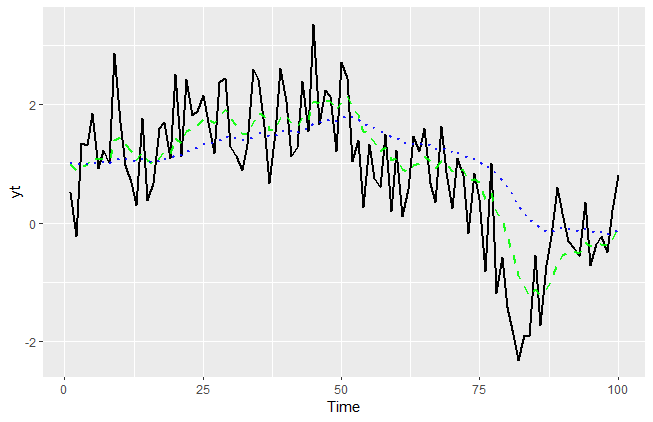
\includegraphics[width=340pt, height=200pt]{Chapters/chapter8/figures/SignaToNoise.png}
	\caption[List of figure caption goes here]{Signal-to-noise ratio: Dynamic linear model.}\label{fig1}
\end{figure} 

Figure \ref{fig1} shows the results of the filtering recursion. We see in this figure that the filtered recursion associated with the high signal-to-noise ratio (green dashed line) follows closer the data than the low signal-to-noise ratio scenario (blue dotted line). We see that the latter is smoother as it gives more weight to the prior mean, which takes into account historical information.

\item Simulate the \textit{dynamic linear model} $y_t=\beta_t x_t + \mu_t$, $\beta_t=\beta_{t-1}+w_t$, where $x_t\sim N(1, 0.1\sigma^2)$, $w_t\sim N(0, 0.5\sigma^2)$, $\mu_t\sim N(0, \sigma^2)$, $\beta_0=0$, $B_0=0.5\sigma^2$, and $\sigma^2=1$, $t=1,\dots,100$. Perform the filtering and smoothing recursions from scratch. 	

\textbf{Answer}

The following code shows how to perform this simulation and perform the filtering recursion from scratch in \textbf{R}. 

\begin{tcolorbox}[enhanced,width=4.67in,center upper,
	fontupper=\large\bfseries,drop shadow southwest,sharp corners]
	\textit{R code. Simulation: Filtering and smoothing recursions from scratch}
	\begin{VF}
		\begin{lstlisting}[language=R]
rm(list = ls()); set.seed(010101)
T <- 100; sig2 <- 1; r <- 0.5; sigW2 <- sig2*r
xt <- rnorm(T, mean = 1, sd = 0.1*sig2^0.5) 
e <- rnorm(T, mean = 0, sd = sig2^0.5)
w <- rnorm(T, mean = 0, sd = sigW2^0.5)
K <- 1; Bt <- matrix(NA, T, K); Bt[1] <- 0
yt <- rep(NA, T)
for(t in 1:T){
	if(t == 1){
		Bt[t,] <- w[t]
	}else{
		Bt[t,] <- Bt[t-1,] + w[t]
	}
	yt[t] <- xt[t]%*%Bt[t,] + e[t]
}
# Filtering
KFR <- function(y, x, b1, B1, Omega, sig2){
	e <- as.numeric(y - t(x)%*%b1) # Error
	R <- B1 + Omega
	q <- as.numeric(t(x)%*%R%*%x + sig2)
	K <- (R%*%x)/q
	bt <- b1 + K*e
	Bt <- R - R%*%x%*%t(x)%*%R/q
	Result <- list(bt = bt, Bt = Bt) 
	return(Result)
}
KFresb <- list(); KFresB <- list()
b0 <- 0; B0 <- sigW2
for(t in 1:T){
	KFrest <- KFR(y = yt[t], x = xt[t], b1 = b0, B1 = B0, Omega = sigW2, sig2 = sig2)
	b0 <- KFrest[["bt"]]; B0 <- KFrest[["Bt"]]
	KFresb[[t]] <- b0; KFresB[[t]] <- B0 
}
ModelReg <- function(par){
	Mod <- dlm::dlmModReg(xt, dV = exp(par[1]), dW = exp(par[2]), m0 = rep(0, K),
	C0 = sigW2*diag(K), addInt = FALSE)
	return(Mod)
}
RegFilter1 <- dlm::dlmFilter(yt, ModelReg(c(sig2, sigW2)))
plot(Bt, type = "l")
lines(unlist(KFresb), type = "l", col = "red")
lines(RegFilter1[["m"]][-1], type = "l", col = "blue")
\end{lstlisting}
	\end{VF}
\end{tcolorbox}

\begin{tcolorbox}[enhanced,width=4.67in,center upper,
	fontupper=\large\bfseries,drop shadow southwest,sharp corners]
	\textit{R code. Simulation: Filtering and smoothing recursions from scratch}
	\begin{VF}
		\begin{lstlisting}[language=R]
# Smoothing 
BSR <- function(b, B, slead, Slead, Omega){
	b = bfilter[t]; B = Bfilter[t]; slead = slead; Slead = slead; Omega = sigW2
	R1 <- B + Omega
	s <- b + B%*%solve(R1)%*%(slead - b)
	S <- B - B%*%solve(R1)%*%(R1 - Slead)%*%solve(R1)%*%B
	Result <- list(st = s, St = S) 
	return(Result)
}
bfilter <- unlist(KFresb); Bfilter <- unlist(KFresB)
slead <- bfilter[T]; Slead <- Bfilter[T]
smooth <- rep(slead, T); Smooth <- rep(Slead, T);  
for(t in (T-1):1){
	BSRrest <- BSR(b = bfilter[t], B = Bfilter[t], slead = slead, Slead = Slead, Omega = sigW2)
	slead <- BSRrest[["st"]]; Slead <- BSRrest[["st"]]
	smooth[t] <- slead
}
RegSmoth <- dlm::dlmSmooth(yt, ModelReg(c(sig2, sigW2)))
VarSmooth <- dlm::dlmSvd2var(u = RegSmoth[["U.S"]], RegSmoth[["D.S"]])
SDVarSmoothB2 <- sapply(2:(T+1), function(t){VarSmooth[[t]][K,K]^0.5}) 
plot(Bt, type = "l")
lines(smooth, type = "l", col = "orange")
lines(RegSmoth[["s"]][-1], type = "l", col = "green")
\end{lstlisting}
	\end{VF}
\end{tcolorbox}


	\item Simulate the process $y_t=\alpha z_t + \beta_t x_t + \bm{h}^{\top}\bm{\epsilon}_t$, $\beta_t=\beta_{t-1}+\bm{H}^{\top}\bm{\epsilon}_t$, where $\bm{h}^{\top}=[1 \ 0]$, $\bm{H}^{\top}=[0 \ 1/\tau]$, $\bm{v}_t\sim N(\bm{0}_2, \sigma^2\bm{I}_2)$, $x_t\sim N(1, 2\sigma^2)$, $z_t\sim N(0, 2\sigma^2)$, $\alpha=2$, $\tau^2=5$ and $\sigma^2=0.1$, $t=1,\dots,200$. Assume $\pi({\beta}_0,{\alpha},\sigma^2,{\tau})=\pi({\beta}_0)\pi({\alpha})\pi(\sigma^2)\pi(\tau^2)$ where $\sigma^2\sim IG(\alpha_0/2,\delta_0/2)$, $\tau^2\sim G(v_{0}/2,v_{0}/2)$, ${\alpha}\sim N({a}_0,{A}_0)$ and ${\beta}_0\sim N({b}_0,{B}_0)$ such that $\alpha_0=\delta_0=1$, $v_0=5$, $a_0=0$, $A_0=1$, $\beta_0=0$, $B_0=\sigma^2/\tau^2$. Program the MCMC algorithm including the \textit{simulation smoother}.
	
	\textbf{Answer}
	

\begin{tcolorbox}[enhanced,width=4.67in,center upper,
	fontupper=\large\bfseries,drop shadow southwest,sharp corners]
	\textit{R code. Simulation: MCMC algorithm with simulation smoother}
	\begin{VF}
		\begin{lstlisting}[language=R]
rm(list = ls()); set.seed(010101)
T <- 200; sig2 <- 0.1; tau2 <- 5; tau <- tau2^0.5; sigW2 <- sig2/tau2
xt <- rnorm(T, mean = 1, sd = 2*sig2^0.5)
zt <- rnorm(T, mean = 1, sd = 2*sig2^0.5)
alpha <- 2
e <- MASS::mvrnorm (T, mu = c(0, 0), Sigma = sig2*diag(2))
K <- 1
h1 <- matrix(c(1, 0), K + 1, 1); h2 <- matrix(c(0, 1/tau), K + 1, 1); t(h1)%*%h2
e1 <- e%*%h1; e2 <- e%*%h2; var(e1); var(e2)
Bt <- matrix(NA, T, K); Bt[1] <- 0
yt <- rep(NA, T) 
for(t in 1:T){
	if(t == 1){
		Bt[t,] <- e2[t]
	}else{
		Bt[t,] <- Bt[t-1,] + e2[t] 
	}
	yt[t] <- zt[t]*alpha + xt[t]*Bt[t] + e1[t]
}
# Recursion functions
# Filter
KFRDSnew <- function(y, z, x, b, B, alpha, tau2){
	e <- as.numeric(y - z*alpha - t(x)%*%b)
	q <- as.numeric(t(x)%*%B%*%x + t(h1)%*%h1)
	K <- (B%*%x)/q
	bt <- b + K*e
	h2 <- matrix(c(0, 1/tau2^0.5))
	Bt <- B - B%*%x%*%t(K) + t(h2)%*%h2
	Result <- list(bt = bt, Bt = Bt, et = e, Kt = K, qt = q) 
	return(Result)
}
# Smooth
BSRDSnew <- function(r, M, Q, e, K, x, sig2, tau2){
	h2 <- matrix(c(0, 1/tau2^0.5))
	Lambda <- t(h2)%*%h2 
	C <- Lambda - Lambda%*%M%*%t(Lambda)
	xi <- rnorm(1, 0, sd = (sig2*C)^0.5)
	L <- 1 - K*x
	V <- Lambda%*%M%*%L
	rtl <- x*e/Q + t(L)*r - t(V)%*%solve(C)%*%xi
	Mtl <- x%*%t(x)/Q + t(L)%*%M%*%L + t(V)%*%solve(C)%*%V
	eta <- Lambda%*%r + xi
	Result <- list(rtl = rtl, Mtl = Mtl, etat = eta)
	return(Result)
}
# Gibbs functions
PostSig2 <- function(bbt, alpha, tau2){
	an <- T*(K + 1) + alpha0
	term1 <- diff(c(0, bbt))
	term2 <- c(yt - alpha*zt - xt*bbt)
	dn <- delta0 + sum(term1^2)*tau2  + sum(term2^2)
	sig2 <- invgamma::rinvgamma(1, shape = an/2, rate = dn/2)
	return(sig2)
}
\end{lstlisting}
	\end{VF}
\end{tcolorbox} 

\begin{tcolorbox}[enhanced,width=4.67in,center upper,
	fontupper=\large\bfseries,drop shadow southwest,sharp corners]
	\textit{R code. Simulation: MCMC algorithm with simulation smoother}
	\begin{VF}
		\begin{lstlisting}[language=R]
PosAlpha <- function(bbt, sig2){
	An <- solve(A0i + sig2^(-1)*t(zt)%*%zt)
	term <- yt-xt*bbt
	an <- An%*%(A0i%*%a0 + sig2^(-1)*t(zt)%*%term)
	Alpha <- MASS::mvrnorm(1, an, An)
	return(Alpha)
}
PostTau2 <- function(bbt, sig2){
	v1n <- v0 + T
	term1 <- diff(c(0,bbt))
	v2n <- v0 + sig2^(-1)*sum(term1^2)
	tau2 <- rgamma(1, v1n/2, v2n/2)
	return(tau2)
}
# Hyperparameter
alpha0 <- 1; delta0 <- 1; v0 <- 5
a0 <- 0; A0 <- 1; A0i <- 1/A0
tau2post <- 2; sig2post <- 0.2; alphapost <- 0
# Inference
S <- 2000; burnin <- 500; tot <- S + burnin; thin <- 5
# Posterior draws
sig2s <- rep(NA, tot); tau2s <- rep(NA, tot)
alphas <- rep(NA, tot); betas <- matrix(NA, tot, T)
pb <- txtProgressBar(min = 0, max = tot, style = 3)
\end{lstlisting}
	\end{VF}
\end{tcolorbox} 

\begin{tcolorbox}[enhanced,width=4.67in,center upper,
	fontupper=\large\bfseries,drop shadow southwest,sharp corners]
	\textit{R code. Simulation: MCMC algorithm with simulation smoother}
	\begin{VF}
		\begin{lstlisting}[language=R]
for (s in 1:tot){
	b0 <- 0; B0 <- sigW2
	KFDSresb <- list(); KFDSresB <- list()
	KFDSresE <- list(); KFDSresK <- list(); KFDSresQ <- list()
	for(t in 1:T){
		KFDSrest <- KFRDSnew(y = yt[t], z = zt[t], x = xt[t], b = b0, B = B0, alpha = alphapost, tau2 = tau2post)
		b0 <- KFDSrest[["bt"]]; B0 <- KFDSrest[["Bt"]]
		KFDSresb[[t]] <- b0; KFDSresB[[t]] <- B0
		KFDSresE[[t]] <- KFDSrest[["et"]]; KFDSresK[[t]] <- KFDSrest[["Kt"]]; KFDSresQ[[t]] <- KFDSrest[["qt"]]
	}
	et <- unlist(KFDSresE); Qt <- unlist(KFDSresQ); Kt <- unlist(KFDSresK)
	rT <- 0; MT <- 0
	BSRDSreseta <- rep(0, T); BSRDSresetaMean <- rep(0, T)
	for(t in (T-1):1){
		BSRDSrest <- BSRDSnew(r = rT, M = MT, Q = Qt[t+1], e = et[t+1], K = Kt[t+1], x = xt[t+1], sig2 = sig2post, tau2 = tau2post)
		rT <- BSRDSrest[["rtl"]]; MT <- BSRDSrest[["Mtl"]]
		BSRDSreseta[t+1] <- BSRDSrest[["etat"]]
	}
	Bt1DSpost <- rep(0,T)
	for(t in 1:T){
		if(t == 1){
			Bt1DSpost[t] <- BSRDSreseta[t]
		}else{
			Bt1DSpost[t] <- Bt1DSpost[t-1] + BSRDSreseta[t]
		}
	}
	sig2post <- PostSig2(bbt = Bt1DSpost, alpha = alphapost, tau2 = tau2post)
	alphapost <- PosAlpha(bbt = Bt1DSpost, sig2 = sig2post)
	tau2post <- PostTau2(bbt = Bt1DSpost, sig2 = sig2post)
	sig2s[s] <- sig2post
	tau2s[s] <- tau2post
	alphas[s] <- alphapost
	betas[s,] <- Bt1DSpost
	setTxtProgressBar(pb, s)
}
close(pb); keep <- seq((burnin+1), tot, thin)
betasF <- betas[keep,]; sig2sF <- coda::mcmc(sig2s[keep])
tau2sF <- coda::mcmc(tau2s[keep]); alphasF <- coda::mcmc(alphas[keep])
summary(sig2sF); plot(sig2sF)
summary(tau2sF); plot(tau2sF)
summary(alphasF); plot(alphasF)
library(fanplot); df <- as.data.frame(betasF)
plot(NULL, main="Percentiles", xlim = c(1, T+1), ylim = c(-4, 1), xlab = "Time", ylab = TeX("$\\beta_{t1}$"))
fan(data = df); lines(colMeans(betasF), col = "black", lw = 2)
lines(Bt, col = "blue")
\end{lstlisting}
	\end{VF}
\end{tcolorbox} 

Figure \ref{fig2} shows the path of the state vector (blue line), and the results from the \textit{simulation smoother} using posterior draws, the black line is the mean, and the red-yellow shadows are different deciles.

\begin{figure}[!h]
	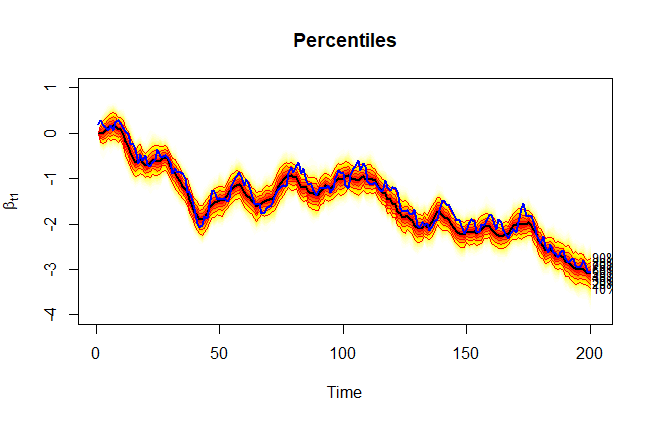
\includegraphics[width=340pt, height=200pt]{Chapters/chapter8/figures/SSfig.png}
	\caption[List of figure caption goes here]{State vector: Dynamic linear model.}\label{fig2}
\end{figure} 

\item Show that the posterior distribution of $\bm{\phi}|\bm{\beta},\sigma^2,\bm{y},\bm{X}$ in the model $Y_t=\bm{x}_t^{\top}\bm{\beta}+\mu_t$ where $\phi(L)\mu_t=\epsilon_t$ and $\epsilon_t\stackrel{iid}{\sim}N(0,\sigma^2)$ is $N(\bm{\phi}_n, \bm{\Phi}_n)\mathbbm{1}[\bm{\phi}\in S_{\bm{\phi}}]$, where $\bm{\Phi}_n=(\bm{\Phi}_0^{-1}+\sigma^{-2}\bm{U}^{\top}\bm{U})$, $\bm{\phi}_n=\bm{\Phi}_n(\bm{\Phi}_0^{-1}\bm{\phi}_0+\sigma^{-2}\bm{U}^{\top}\bm{\mu})$, and $S_{\phi}$ is the stationary region of $\bm{\phi}$.
	
\textbf{Answer}
	
The conditional posterior distribution can be got as follows:
	\begin{align*}
		\pi(\bm{\phi}|\bm{\beta},\sigma^2,\bm{y})&\propto \exp\left\{-\frac{1}{2\sigma^2}(\bm{\mu}-\bm{U}\bm{\phi})^{\top}(\bm{\mu}-\bm{U}\bm{\phi})\right\}\\
		&\times \exp\left\{-\frac{1}{2}(\bm{\phi}-\bm{\phi}_0)^{\top}\bm{\Phi}_0^{-1}(\bm{\phi}-\bm{\phi}_0)\right\}\\
		&\propto\exp\left\{-\frac{1}{2}[\bm{\phi}^{\top}(\sigma^{-2}\bm{U}^{\top}\bm{U}+\bm{\Phi}_0^{-1})\bm{\phi}-2\bm{\phi}^{\top}(\sigma^{-2}\bm{U}^{\top}\bm{\mu}+\bm{\Phi}_0^{-1}\bm{\phi}_0)\right.\\
		&\left.+\bm{\phi}_n^{\top}\bm{\Phi}_n^{-1}\bm{\phi}_n-\bm{\phi}_n^{\top}\bm{\Phi}_n^{-1}\bm{\phi}_n]\right\}\\
		&\propto\exp\left\{-\frac{1}{2}[(\bm{\phi}-\bm{\phi}_n)^{\top}\bm{\Phi}_n^{-1}(\bm{\phi}-\bm{\phi}_n)]\right\}, 
	\end{align*}
where $\bm{\Phi}_n=(\sigma^{-2}\bm{U}^{\top}\bm{U}+\bm{\Phi}_0^{-1})^{-1}$ and $\bm{\phi}_n=\bm{\Phi}_n(\sigma^{-2}\bm{U}^{\top}\bm{\mu}+\bm{\Phi}_0^{-1}\bm{\phi}_0)$. The last expression is the kernel of a multivariate normal distribution with mean $\bm{\phi}_n$ and variance matrix $\bm{\Phi}_n$.   

	\item Show that in the $AR(2)$ stationary process, $Y_t=\mu+\phi_1Y_{t-1}+\phi_2Y_{t-2}+\epsilon_t$, where $\epsilon_t\sim N(0,\sigma^2)$, $\mathbb{E}[Y_t]=\frac{\mu}{1-\phi_1-\phi_2}$, and $Var[Y_t]=\frac{\sigma^2(1-\phi_2)}{1-\phi_2-\phi_1^2-\phi_1^2\phi_2-\phi_2^2+\phi_2^3}$.

\textbf{Answer}

A necessary condition to achieve second-order stationarity in the $AR(2)$ process is that roots of of the polynomial $1-\phi_1L-\phi_2L^2=0$ lie outside the unit circle. This is achieved if $|\phi_2|<1$, $\phi_1+\phi_2<1$ and $\phi_2-\phi_1<1$.

Let's calculate the expected value:
\begin{align*}
	\mathbb{E}[Y_t]&=\bar{\mu}\\
	&=\mathbb{E}[\mu+\phi_1Y_{t-1}+\phi_2Y_{t-2}+\epsilon_t]\\
	&=\mu+\phi_1\mathbb{E}[Y_{t-1}]+\phi_2\mathbb{E}[Y_{t-2}]+\mathbb{E}[\epsilon_{t}]\\
	&=\mu+\phi_1\bar{\mu}+\phi_2\bar{\mu},
\end{align*}
then, $\bar{\mu}(1-\phi_1-\phi_2)=\mu$, then, $\mathbb{E}[Y_t]=\bar{\mu}=\frac{\mu}{1-\phi_1-\phi_2}$.

See that $Y_t=\mu+\phi_1Y_{t-1}+\phi_2Y_{t-2}+\epsilon_t$ implies that $Y_t=\bar{\mu}(1-\phi_1-\phi_2)+\phi_1Y_{t-1}+\phi_2Y_{t-2}+\epsilon_t$, which means that $Y_t-\bar{\mu}=\phi_1(Y_{t-1}-\bar{\mu})+\phi_2(Y_{t-2}-\bar{\mu})+\epsilon_t$, and setting $z_t=Y_t-\bar{\mu}$, we have $z_t=\phi_1z_{t-1}+\phi_2z_{t-2}+\epsilon_t$ where $\mathbb{E}[z_t]=0$. Then, we can calculate the variance of $Y_t$ using $z_t$, given that both have same variance.  

Let's define $\gamma_s=Cov(z_t,z_{t-s})=\mathbb{E}[z_tz_{t-s}]$, then the Yule-Walker equations are:
\begin{align*}
	\gamma_0&=\phi_1\gamma_1+\phi_2\gamma_2+\sigma^2\\
	\gamma_1&=\phi_1\gamma_0+\phi_2\gamma_1\\
	\gamma_2&=\phi_1\gamma_1+\phi_2\gamma_0.
\end{align*}  
Solving this system of equations for $\gamma_0$, $\gamma_1$ and $\gamma_2$, we find that $\gamma_0=\frac{\sigma^2(1-\phi_2)}{1-\phi_2-\phi_1^2-\phi_1^2\phi_2-\phi_2^2+\phi_2^3}$.

\item Program a Hamiltonian Monte Carlo (HMC) taking into account the stationary restrictions on $\phi_1$ and $\phi_2$, and $\epsilon_0$ such that the acceptance rate is near 65\%.

\textbf{Answer}

We know from the previous exercise that $|\phi_2|<1$, $\phi_1+\phi_2<1$ and $\phi_2-\phi_1<1$ satisfied the stationary condition of the process. Thus, we should impose this restrictions in the HMC. The following code does this.

\begin{tcolorbox}[enhanced,width=4.67in,center upper,
	fontupper=\large\bfseries,drop shadow southwest,sharp corners]
	\textit{R code. AR(2) model:  Hamiltonian Monte Carlo with stationary restrictions}
	\begin{VF}
		\begin{lstlisting}[language=R]
# Simulation AR(2)
rm(list = ls()); set.seed(010101); T <- 1000; K <- 4 
mu <- 0.5; phi1 <- 0.5; phi2 <- 0.3; sig <- 0.5 
Ey <- mu/(1-phi1-phi2); Sigy <- sig*((1-phi2)/(1-phi2-phi1^2-phi2*phi1^2-phi2^2+phi2^3))^0.5 
y <- rnorm(T, mean = Ey, sd = Sigy); e <- rnorm(T, mean = 0, sd = sig)
for(t in 3:T){
	y[t] <- mu + phi1*y[t-1] + phi2*y[t-2] + e[t]
}
# Hyperparameters
d0 <- 0.01; a0 <- 0.01; mu0 <- 0; MU0 <- 1
phi0 <- c(0, 0); Phi0 <- diag(2)
# Log posterior multiply by -1 to use optim
LogPost <- function(theta, y){
	mu <- theta[1]; phi1 <- theta[2]; phi2 <- theta[3]
	tau <- theta[4]; sig2 <- exp(tau); logLik <- NULL
	for(t in 3:T){
		logLikt <- dnorm(y[t], mean = mu + phi1*y[t-1] + phi2*y[t-2], sd = sig2^0.5, log = TRUE)
		logLik <- c(logLik, logLikt)
	}
	logLik <- sum(logLik)
	logPrior <- dnorm(mu, mean = mu0, sd = MU0^0.5, log = TRUE) + dnorm(phi1, mean = phi0[1], sd = Phi0[1,1]^0.5, log = TRUE) + dnorm(phi2, mean = phi0[2], sd = Phi0[2,2]^0.5, log = TRUE) + invgamma::dinvgamma(sig2, shape = a0/2, rate = d0/2, log = TRUE)
	logPosterior <- logLik + logPrior + tau
	return(-logPosterior) # Multiply by -1 to minimize using optim
}
theta0 <- c(mean(y), 0, 0, var(y))
Opt <- optim(theta0, LogPost, y = y, hessian = TRUE)
theta0 <- Opt$par; VarPost <- solve(Opt$hessian)
# Gradient log posterior
GradientTheta <- function(theta, y){
	mu <- theta[1]; phi1 <- theta[2]; phi2 <- theta[3]
	tau <- theta[4]; sig2 <- exp(tau); SumLik <- matrix(0, 3, 1)
	SumLik2 <- NULL
	for(t in 3:T){
		xt <- matrix(c(1, y[t-1], y[t-2]), 3, 1)
		SumLikt <- (y[t] - (mu + phi1*y[t-1] + phi2*y[t-2]))*xt
		SumLik2t <- (y[t] - (mu + phi1*y[t-1] + phi2*y[t-2]))^2
		SumLik <- rowSums(cbind(SumLik, SumLikt))
		SumLik2 <- sum(SumLik2, SumLik2t)
	}
	Grad_mu <- SumLik[1]/sig2 - (1/MU0)*(mu - mu0)
	Grad_phi1 <- SumLik[2]/exp(tau) - 1/Phi0[1,1]*(phi1 - phi0[1])
	Grad_phi2 <- SumLik[3]/exp(tau) - 1/Phi0[2,2]*(phi2 - phi0[2])
	Grad_tau <- -(T-2)/2 + SumLik2/(2*exp(tau)) - (a0/2 + 1) + d0/(2*exp(tau)) + 1 
	Grad <- c(Grad_mu, Grad_phi1, Grad_phi2, Grad_tau)
	return(Grad)
}
\end{lstlisting}
	\end{VF}
\end{tcolorbox} 

\begin{tcolorbox}[enhanced,width=4.67in,center upper,
	fontupper=\large\bfseries,drop shadow southwest,sharp corners]
	\textit{R code. AR(2) model:  Hamiltonian Monte Carlo with stationary restrictions}
	\begin{VF}
		\begin{lstlisting}[language=R]
StatRest <- function(phi1, phi2){
	if(abs(phi2) < 1 & phi1 + phi2 < 1 & phi2 - phi1 < 1){
		check <- 1
	}else{
		check <- 0
	}
	return(check)
}
HMC <- function(theta, y, epsilon, M){
	L <- ceiling(1/epsilon)
	Minv <- solve(M)
	thetat <- theta
	K <- length(thetat)
	mom <- t(mvtnorm::rmvnorm(1, rep(0, K), M))
	logPost_Mom_t <- -LogPost(thetat, y) +  mvtnorm::dmvnorm(t(mom), rep(0, K), M, log = TRUE)  
	for(l in 1:L){
		if(l == L){
			mom <- mom + 0.5*epsilon*GradientTheta(theta, y)
			theta <- theta + epsilon*Minv%*%mom
		}else{
			mom <- mom + epsilon*GradientTheta(theta, y)
			theta <- theta + epsilon*Minv%*%mom
		}
	}
	logPost_Mom_star <- -LogPost(theta, y) +  mvtnorm::dmvnorm(t(mom), rep(0, K), M, log = TRUE)  
	alpha <- min(1, exp(logPost_Mom_star-logPost_Mom_t))
	u <- runif(1)
	if(u <= alpha & StatRest(phi1 = theta[2], phi2 = theta[3]) == 1){
		thetaNew <- c(theta)
	}else{
		thetaNew <- thetat
	}
	rest <- list(theta = thetaNew, Prob = alpha)
	return(rest)
}
\end{lstlisting}
	\end{VF}
\end{tcolorbox}     


\begin{tcolorbox}[enhanced,width=4.67in,center upper,
	fontupper=\large\bfseries,drop shadow southwest,sharp corners]
	\textit{R code. AR(2) model:  Hamiltonian Monte Carlo with stationary restrictions}
	\begin{VF}
		\begin{lstlisting}[language=R]
# Posterior draws
S <- 1000; burnin <- 1000; thin <- 2; tot <- S + burnin
thetaPost <- matrix(NA, tot, K)
ProbAcept <- rep(NA, tot)
# theta0 <- theta0
theta0 <- c(mean(y), 0, 0, exp(var(y)))  
M <- solve(VarPost); epsilon0 <- 0.4
pb <- txtProgressBar(min = 0, max = tot, style = 3)
for(s in 1:tot){
	epsilon <- runif(1, 0, 2*epsilon0)
	L <- ceiling(1/epsilon)
	HMCs <- HMC(theta = theta0, y, epsilon, M) 
	theta0 <- HMCs$theta 
	thetaPost[s,] <- HMCs$theta
	ProbAcept[s] <- HMCs$Prob
	setTxtProgressBar(pb, s)
}
close(pb)
keep <- seq((burnin+1), tot, thin)
thetaF <- coda::mcmc(thetaPost[keep,])
summary(thetaF)
plot(thetaF)
summary(exp(thetaF[,K]))
plot(exp(thetaF[,K]))
ProbAceptF <- coda::mcmc(ProbAcept[keep])
summary(ProbAceptF)
\end{lstlisting}
	\end{VF}
\end{tcolorbox}  

\item \textbf{Stochastic volatility model}
\begin{itemize}
	\item Program a sequential importance sampling (SIS) from scratch in the vanilla stochastic volatility model setting $\mu=-10$, $\phi = 0.95$, $\sigma=0.3$ and $T=250$. Check what happen with its performance.
	\item Modify the sequential Monte Carlo (SMC) to perform multinomial resampling when the effective sample size is lower than 50\% the number of particles.  
\end{itemize}

\textbf{Answer}

We observe that, initially, sequential importance sampling performs relatively well. However, particle degeneracy occurs around $(t=50)$, causing the algorithm's performance to deteriorate rapidly (see Figure \ref{figSIS}). We can see in Figure \ref{figESS} how the effective sample size (ESS) of the particles decreases rapidly.

\begin{tcolorbox}[enhanced,width=4.67in,center upper,
	fontupper=\large\bfseries,drop shadow southwest,sharp corners]
	\textit{R code. Stochastic volatility model:  Sequential importance sampling}
	\begin{VF}
		\begin{lstlisting}[language=R]
rm(list = ls()); set.seed(010101)
T <- 250; K <- 2; mu <- -10; phi <- 0.95; sigma <- 0.3
h <- numeric(T); y <- numeric(T)
h[1] <- rnorm(1, mu, sigma / sqrt(1 - phi^2))
y[1] <- rnorm(1, 0, exp(h[1] / 2))
for (t in 2:T) {
	h[t] <- mu + phi*(h[t-1]-mu) + rnorm(1, 0, sigma)
	y[t] <- rnorm(1, 0, sd = exp(0.5*h[t]))
}
N <- 10000
log_Weights <- matrix(NA, N, T)  # Log weights
Weights <- matrix(NA, N, T)  # Weights 
WeightsST <- matrix(NA, N, T)  # Normalized weights 
particles <- matrix(NA, N, T)   # Particles
logalphas <- matrix(NA, N, T)   # Incremental importance weights
ESS <- rep(NA, T) # Effective sample size
particles[, 1] <- rnorm(N, mu, sigma / sqrt(1 - phi^2))
log_Weights[, 1] <- dnorm(y[1], 0, sd = exp(0.5*particles[,1]), log = TRUE)  
Weights[, 1] <- exp(log_Weights[, 1])
WeightsST[, 1] <- Weights[, 1] / sum(Weights[, 1])
ESS[1] <- (sum(WeightsST[, 1]^2))^(-1)
for (t in 2:T) {
	particles[, t] <- rnorm(N, mu + phi*(particles[, t - 1] - mu), sigma)  # Sample from proposal
	logalphas[, t] <- dnorm(y[t], 0, sd = exp(0.5*particles[,t]), log = TRUE) 
	log_Weights[, t] <- log_Weights[, t - 1] + logalphas[, t]
	Weights[, t] <- exp(log_Weights[, t])
	WeightsST[, t] <- Weights[, t] / sum(Weights[, t])
	ESS[t] <- (sum(WeightsST[, t]^2))^(-1)
}
FilterDist <- colSums(particles * WeightsST)
SDFilterDist <- (colSums(particles^2 * WeightsST) - FilterDist^2)^0.5
MargLik <- colMeans(Weights)
library(dplyr); library(ggplot2); require(latex2exp)
ggplot2::theme_set(theme_bw())
df <- tibble(t = seq(1, T), mean = FilterDist, lower = FilterDist - 1.96*SDFilterDist, upper = FilterDist + 1.96*SDFilterDist, x_true = h)
plot_filtering_estimates <- function(df) {
	p <- ggplot(data = df, aes(x = t)) + geom_ribbon(aes(ymin = lower, ymax = upper), alpha = 1, fill = "lightblue") + geom_line(aes(y = x_true), colour = "black", alpha = 1, linewidth = 0.5) + geom_line(aes(y = mean), colour = "blue", linewidth = 0.5) +
	ylab(TeX("$h_{t}$")) + xlab("Time")
	print(p)
}
plot_filtering_estimates(df)
plot(ESS, type = "l", ylab = "Effective sample size", xlab = "Time")
\end{lstlisting}
	\end{VF}
\end{tcolorbox} 

\begin{figure}[!h]
	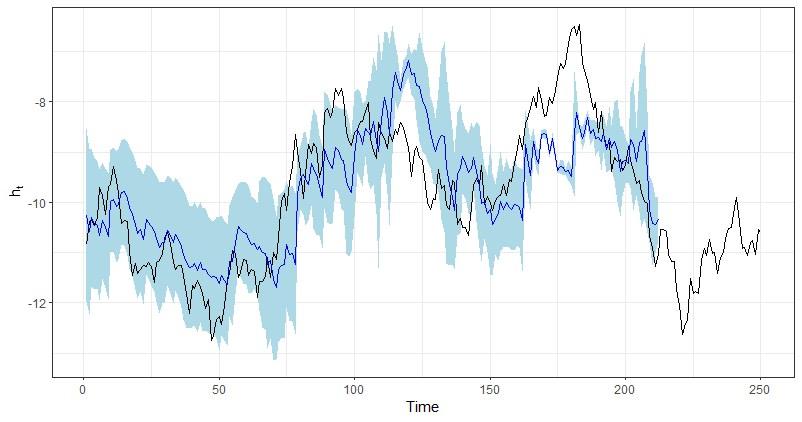
\includegraphics[width=340pt, height=200pt]{Chapters/chapter8/figures/SIS.png}
	\caption[List of figure caption goes here]{Stochastic volatility model: Sequential importance sampling (SIS).}\label{figSIS}
\end{figure}

\begin{figure}[!h]
	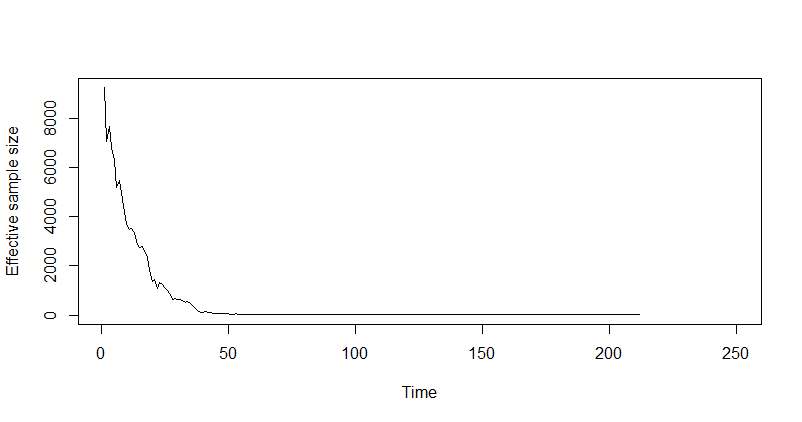
\includegraphics[width=340pt, height=200pt]{Chapters/chapter8/figures/ESSsis.png}
	\caption[List of figure caption goes here]{Stochastic volatility model: Effective sample size (ESS) of the particles.}\label{figESS}
\end{figure} 

This code shows how to program the SMC algorithm performing multinomial resampling when the effective sample size es lower than 50\% the initial number of particles. It seems that in this example is better to perform resampling every time period as the mean recursion (blue and purple lines) are not good following in state (black line). However, the bands corresponding to plus/minus two standard deviations (light blue shading) encompass the state vector; although, it is too wide.

\begin{tcolorbox}[enhanced,width=4.67in,center upper,
	fontupper=\large\bfseries,drop shadow southwest,sharp corners]
	\textit{R code. Stochastic volatility model: Sequential Monte Carlo}
	\begin{VF}
		\begin{lstlisting}[language=R]
rm(list = ls()); set.seed(010101)
T <- 1250; mu <- -10; phi <- 0.95; sigma <- 0.3
h <- numeric(T); y <- numeric(T)
h[1] <- rnorm(1, mu, sigma / sqrt(1 - phi^2))  
y[1] <- rnorm(1, 0, exp(h[1] / 2))          
for (t in 2:T) {
	h[t] <- mu + phi*(h[t-1]-mu) + rnorm(1, 0, sigma)
	y[t] <- rnorm(1, 0, sd = exp(0.5*h[t]))
}
N <- 10000
log_Weights <- matrix(NA, N, T)  # Log weights
Weights <- matrix(NA, N, T)  # Weights 
WeightsST <- matrix(NA, N, T)  # Normalized weights 
WeightsSTT <- matrix(1/N, N, T)  # Normalized weights bar 
particles <- matrix(NA, N, T)   # Particles
particlesT <- matrix(NA, N, T)   # Particles bar
logalphas <- matrix(NA, N, T)   # Incremental import. weig.
ESS <- rep(NA, T) # Efective sample size
cutoff <- 0.5
particles[, 1] <- rnorm(N, mu, sigma / sqrt(1 - phi^2)) 
log_Weights[, 1] <- dnorm(y[1], 0, sd = exp(0.5*particles[,1]), log = TRUE)  
Weights[, 1] <- exp(log_Weights[, 1])
WeightsST[, 1] <- Weights[, 1] / sum(Weights[, 1])
ESS[1] <- (sum(WeightsST[, 1]^2))^(-1)
ind <- sample(1:N, size = N, replace = TRUE, prob = WeightsST[, 1]) # Resample 
particles[, 1] <- particles[, 1] # Resampled particles
particlesT[, 1] <- particles[ind, 1] # Resampled particles
WeightsST[, 1] <- rep(1/N, N) # Resampled weights
pb <- txtProgressBar(min = 0, max = T, style = 3)
for (t in 2:T) {
	particles[, t] <- rnorm(N, mu + phi*(particles[, t - 1] - mu), sigma)  # Sample from proposal
	logalphas[, t] <- dnorm(y[t], 0, sd = exp(0.5*particles[,t]), log = TRUE) 
	Weights[, t] <- exp(logalphas[, t])
	WeightsST[, t] <- Weights[, t] / sum(Weights[, t])
	ESS[t] <- (sum(WeightsST[, t]^2))^(-1)
	particlesT[, t] <- particles[, t]
	if(ESS[t] < N*cutoff){
		ind <- sample(1:N, size = N, replace = TRUE, prob = WeightsST[, t])
		particles[, 1:t] <- particles[ind, 1:t]
		WeightsST[, t] <- 1/N
	}else{if(t == T & ESS[t] < N*cutoff)
		ind <- sample(1:N, size = N, replace = TRUE, prob = WeightsST[, t])
		particlesT[, 1:t] <- particles[ind, 1:t]
	}
	setTxtProgressBar(pb, t)
}
close(pb)
\end{lstlisting}
	\end{VF}
\end{tcolorbox} 

\begin{tcolorbox}[enhanced,width=4.67in,center upper,
	fontupper=\large\bfseries,drop shadow southwest,sharp corners]
	\textit{R code. Stochastic volatility model: Sequential Monte Carlo}
	\begin{VF}
		\begin{lstlisting}[language=R]
FilterDist <- colSums(particles * WeightsST)
SDFilterDist <- (colSums(particles^2 * WeightsST) - FilterDist^2)^0.5
FilterDistT <- colSums(particlesT * WeightsSTT)
SDFilterDistT <- (colSums(particlesT^2 * WeightsSTT) - FilterDistT^2)^0.5
MargLik <- colMeans(Weights)
plot(MargLik, type = "l")
plot(ESS, type = "l")
library(dplyr)
library(ggplot2)
require(latex2exp)
ggplot2::theme_set(theme_bw())
Tfig <- 250
keepFig <- 1:Tfig
df <- tibble(t = keepFig,
mean = FilterDist[keepFig],
lower = FilterDist[keepFig] - 2*SDFilterDist[keepFig],
upper = FilterDist[keepFig] + 2*SDFilterDist[keepFig],
meanT = FilterDistT[keepFig],
lowerT = FilterDistT[keepFig] - 2*SDFilterDistT[keepFig],
upperT = FilterDistT[keepFig] + 2*SDFilterDistT[keepFig],
x_true = h[keepFig])
plot_filtering_estimates <- function(df) {
	p <- ggplot(data = df, aes(x = t)) +
	geom_ribbon(aes(ymin = lower, ymax = upper), alpha = 1,
	fill = "lightblue") +
	geom_line(aes(y = x_true), colour = "black", alpha = 1,
	linewidth = 0.5) +
	geom_line(aes(y = mean), colour = "blue", linewidth = 0.5) +
	geom_line(aes(y = meanT), colour = "purple", linewidth = 0.5) +
	ylab(TeX("$h_{t}$")) + xlab("Time")
	print(p)
}
plot_filtering_estimates(df)
\end{lstlisting}
	\end{VF}
\end{tcolorbox} 

\begin{figure}[!h]
	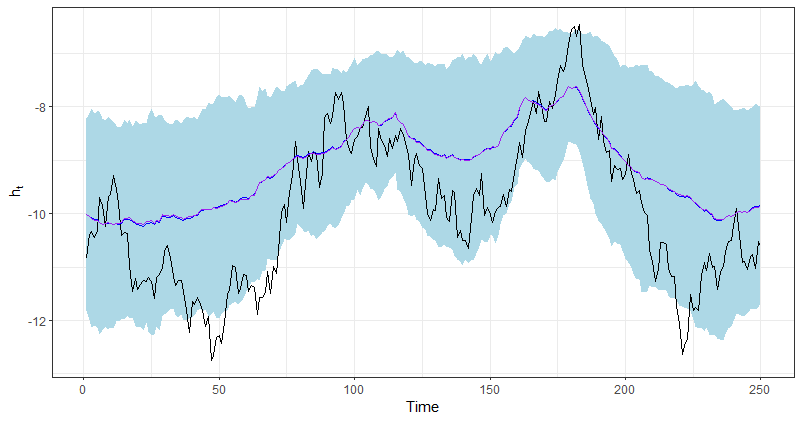
\includegraphics[width=340pt, height=200pt]{Chapters/chapter8/figures/SMCsv_resam}
	\caption[List of figure caption goes here]{Stochastic volatility model: Sequential Monte Carlo (SMC).}\label{fig5}
\end{figure}

\item Estimate the vanilla stochastic volatility model using the dataset \textit{17ExcRate.csv} provided by \cite{ramirez2024testing} of the exchange rate log daily returns from USD/EUR, USD/GBP and GBP/EUR one year before and after the WHO declared the COVID-19 pandemic on 11 March 2020. 

\textbf{Answer}

The following code shows the results of modeling the exchange rate log daily returns from USD/EUR using a stochastic volatility model. Similar code can be used to estimate the other two models.

\begin{tcolorbox}[enhanced,width=4.67in,center upper,
	fontupper=\large\bfseries,drop shadow southwest,sharp corners]
	\textit{R code. Stochastic volatility model: Exchange rate log daily returns from USD/EUR}
	\begin{VF}
		\begin{lstlisting}[language=R]
rm(list = ls()); set.seed(010101)
DataExcRate <- read.csv("https://raw.githubusercontent.com/besmarter/BSTApp/refs/heads/master/DataApp/17ExcRate.csv", sep = ",", header = TRUE, quote = "")
attach(DataExcRate)
MCMC <- 10000; burnin <- 10000; thin <- 5
y <- USDEUR - mean(USDEUR)
plot(y, type = "l")
res <- stochvol::svsample(y, draws = MCMC, burnin = burnin, thin = thin, priormu = c(0, 100), priorsigma = c(1), priorphi = c(5, 1.5), priorbeta =  c(0, 10000))
summary(res[["para"]][[1]][,-c(4,5)])
Iterations = 10005:20000
Thinning interval = 5 
Number of chains = 1 
Sample size per chain = 2000 
1. Empirical mean and standard deviation for each variable,
plus standard error of the mean:
Mean      SD  Naive SE Time-series SE
mu    -11.2886 0.28916 0.0064657       0.006466
phi     0.9618 0.02202 0.0004923       0.001421
sigma   0.1664 0.04501 0.0010064       0.003722
2. Quantiles for each variable:
				2.5%      25%      50%      75%    97.5%
mu    -11.81067 -11.4287 -11.2902 -11.1448 -10.7699
phi     0.90719   0.9512   0.9657   0.9774   0.9913
sigma   0.09615   0.1327   0.1607   0.1926   0.2666
plot(res)
ht <- res[["latent"]][[1]]
library(dplyr)
library(ggplot2)
require(latex2exp)
ggplot2::theme_set(theme_bw())
x_means <- colMeans(ht)
x_quantiles <- apply(ht, 2, function(x) quantile(x, probs = c(0.025, 0.975)))
df <- tibble(t = 1:length(y),
mean = x_means,
lower = x_quantiles[1, ],
upper = x_quantiles[2, ])
plot_filtering_estimates <- function(df) {
	p <- ggplot(data = df, aes(x = t)) +
	geom_ribbon(aes(ymin = lower, ymax = upper), alpha = 1,
	fill = "lightblue") +
	geom_line(aes(y = mean), colour = "blue", linewidth = 0.5) +
	ylab(TeX("$h_{t}$")) + xlab("Time")
	print(p)
}
plot_filtering_estimates(df)
\end{lstlisting}
	\end{VF}
\end{tcolorbox} 

\begin{figure}[!h]
	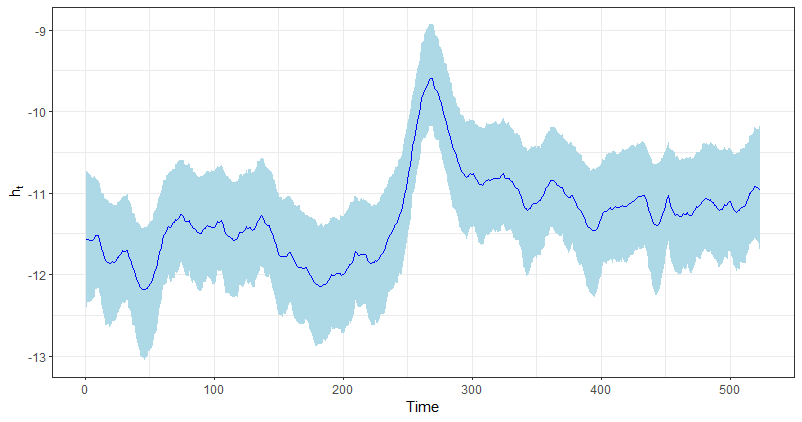
\includegraphics[width=340pt, height=200pt]{Chapters/chapter8/figures/SVUSD_EURO}
	\caption[List of figure caption goes here]{Stochastic volatility model: Exchange rate log daily returns from USD/EUR.}\label{fig6}
\end{figure}

	\item Simulate the VAR(1) process
\begin{align*}
	\begin{bmatrix}
		y_{1t}\\
		y_{2t}\\
		y_{3t}\\
	\end{bmatrix} = \begin{bmatrix}
		2.8\\
		2.2\\
		1.3\\
	\end{bmatrix} + \begin{bmatrix}
		0.5 & 0 & 0\\
		0.1 & 0.1 & 0.3\\
		0 & 0.2 & 0.3\\
	\end{bmatrix} \begin{bmatrix}
		y_{1t-1}\\
		y_{2t-1}\\
		y_{3t-1}\\
	\end{bmatrix} +\begin{bmatrix}
		\mu_{1t}\\
		\mu_{2t}\\
		\mu_{3t}\\
	\end{bmatrix},
\end{align*}
where $\bm{\Sigma}= \begin{bmatrix}
	2.25 & 0 & 0\\
	0 & 1 & 0.5\\
	0 & 0.5 & 0.74\\
\end{bmatrix}$.

\begin{itemize}
	\item  Use vague independent priors setting $\bm{\beta}_0=\bm{0}$, $\bm{B}_0=100\bm{I}$, $\bm{V}_0=5\bm{I}$ and $\alpha_0=3$, and estimate a VAR(1) model using the \textit{rsurGibbs} function from the package \textit{bayesm}. Then, program from scratch algorithms to perform inference of the \textit{forecast error} and \textit{ortogonalized} impulse response functions, and compare with the population impulse response functions, that is, using the population parameters.
	
	\item Using the previous setting perform inference of the \textit{forecast error} and the \textit{ortogonalized} impulse responses using the package \textit{bvartools}.  
\end{itemize}

\textbf{Answer}

Using the recursion $\bm{\Phi}_s=\sum_{l=1}^s\bm{\Phi}_{s-l}\bm{A}_l$, $\bm{A}_l=\bm{0}$, $l>p$ and $s=1,2,..$, we get $\bm{\Phi}_s = \bm{A}_1^s$. In addition, we know that $\bm{\Theta}_s=\bm{\Phi}_S\bm{P}$. Then, we can get these impulse response functions. 

The following code shows how to perform from scratch the impulse response functions. Figure \ref{fig7} shows the \textit{forecast error impulse response} of $y_{2t}$ to shocks in $\mu_{3t}$. We see that the 95\% (blue shadow) and 90\% (light blue shadow) credible intervals of the impulse response functions embrace the true impulse response (black line); although the mean impulse response (blue line) overestimates the true impulse. In addition, we can see that the results from the \textit{bvartools} package have the same patterns compared to the ones that we get programming the algorithm from scratch. Remember that the \textit{bvartools} package uses the inverse Wishart distribution as prior for $\bm{\Sigma}$, where the hyperparameters are the degrees of freedom of the error term, and the prior error variance of endogenous variables.   

\begin{tcolorbox}[enhanced,width=4.67in,center upper,
	fontupper=\large\bfseries,drop shadow southwest,sharp corners]
	\textit{R code. Vector autoregressive model: Simulation}
	\begin{VF}
		\begin{lstlisting}[language=R]
rm(list = ls()); set.seed(010101)
T <- 300; M <- 3
SIGMA <- matrix(c(2.25, 0, 0, 0, 1, 0.5, 0, 0.5, 0.74), M, M )
U <- MASS::mvrnorm(T, rep(0, M), SIGMA)
A <- matrix(c(0.5, 0.1, 0, 0, 0.1, 0.2, 0, 0.3, 0.3), M, M ) 
v <- c(1.4, 1.9, 1.1); Y <- matrix(NA, T, M)
Y[1, ] <- solve(diag(M)-A)%*%v + U[1,]
for(t in 2:T){
	Y[t, ] <- v + A%*%Y[t-1,] + U[t,]
}
plot(Y[,1], type = "l"); plot(Y[,2], type = "l"); plot(Y[,3], type = "l")
y1 <- Y[-1,1]; y2 <- Y[-1,2]; y3 <- Y[-1,3]
X1 <- cbind(1, lag(Y)); X1 <- X1[-1,]
X2 <- cbind(1, lag(Y)); X2 <- X2[-1,]
X3 <- cbind(1, lag(Y)); X3 <- X3[-1,]
regdata <- NULL
regdata[[1]] <- list(y = y1, X = X1); regdata[[2]] <- list(y = y2, X = X2); regdata[[3]] <- list(y = y3, X = X3)
M <- length(regdata); K1 <- dim(X1)[2]; K2 <- dim(X2)[2]; K3 <- dim(X3)[2] 
K <- K1 + K2 + K3
# Hyperparameters
b0 <- rep(0, K); c0 <- 100
B0 <- c0*diag(K); V <- 5*diag(M); a0 <- M
Prior <- list(betabar = b0, A = solve(B0), nu = a0, V = V)
#Posterior draws
MCMC <- 10000; thin <- 5; burnin <- 1000; tot <- MCMC + burnin
Mcmc <- list(R = tot, keep = thin)
PosteriorDraws <- bayesm::rsurGibbs(Data = list(regdata = regdata), Mcmc = Mcmc, Prior = Prior)
keep <- seq(round(burnin/thin)+1, round(tot/thin))
Bs <- PosteriorDraws[["betadraw"]][keep,]
SIGMAs <- PosteriorDraws[["Sigmadraw"]][keep,] 
S <- dim(Bs)[1]
As <- array(NA, c(M, M, S))
for(s in 1:S){
	As[,,s] <- matrix(Bs[s, -c(1, 5, 9)], M, M, byrow = TRUE)
}
# Impulse response functions
H <- 10; Ptrue <- t(chol(SIGMA))
Phistrue <-  array(NA, c(M, M, H))
Phistrue[,,1] <- diag(M); PhistrueAccum <-  Phistrue
PhistrueAccum[,,1] <- diag(M)
Thetastrue <- Phistrue; Thetastrue[,,1] <- Ptrue
ThetastrueAccum <-  Thetastrue; ThetastrueAccum[,,1] <- Ptrue
for(h in 2:H){
	Phistrue[,,h] <- Phistrue[,,h-1]%*%A
	PhistrueAccum[,,h] <- PhistrueAccum[,,h-1] + Phistrue[,,h]
	Thetastrue[,,h] <- Phistrue[,,h]%*%Ptrue
	PhistrueAccum[,,h] <- ThetastrueAccum[,,h-1] + Thetastrue[,,h]
}
P <- array(NA, c(M, M, S))
\end{lstlisting}
	\end{VF}
\end{tcolorbox} 

\begin{tcolorbox}[enhanced,width=4.67in,center upper,
	fontupper=\large\bfseries,drop shadow southwest,sharp corners]
	\textit{R code. Vector autoregressive model: Simulation}
	\begin{VF}
		\begin{lstlisting}[language=R]
for(s in 1:S){
	P[,,s] <- t(chol(matrix(SIGMAs[s,], M, M))) 
}
Phis <- list(); PhisAcum <- list() 
Thetas <- list(); ThetasAcum <- list()
for(h in 0:H){
	if(h == 0){
		Phis[[h+1]] <- array(diag(M), c(M,M,S))
		Thetas <- Phis
		for(s in 1:S){
			Thetas[[h+1]][,,s] <- Phis[[h+1]][,,s]%*%P[,,s]
		}
		PhisAcum[[h+1]] <- Phis[[h+1]]
		ThetasAcum[[h+1]] <- Thetas[[h+1]]
	}else{
		Phis[[h+1]] <- array(diag(M), c(M,M,S))
		Thetas[[h+1]] <- Phis[[h+1]]
		for(s in 1:S){
			Phis[[h+1]][,,s] <- Phis[[h]][,,s]%*%As[,,s]
			Thetas[[h+1]][,,s] <- Phis[[h+1]][,,s]%*%P[,,s]
		}
		PhisAcum[[h+1]] <- PhisAcum[[h]] + Phis[[h+1]]
		ThetasAcum[[h+1]] <- ThetasAcum[[h]] + Thetas[[h+1]]
	}
}
library(dplyr); library(ggplot2); require(latex2exp)
ggplot2::theme_set(theme_bw())
plot_filtering_estimates <- function(df) {
	p <- ggplot(data = df, aes(x = t)) +
	geom_ribbon(aes(ymin = lower1, ymax = upper1), alpha = 1,
	fill = "blue") +
	geom_ribbon(aes(ymin = lower, ymax = upper), alpha = 1,
	fill = "lightblue") +
	geom_line(aes(y = x_true), colour = "black", alpha = 1,
	linewidth = 0.5) +
	geom_line(aes(y = mean), colour = "blue", linewidth = 0.5) +
	ylab("Impulse response") + xlab("Time") + xlim(0,H-1)
	print(p)
}
\end{lstlisting}
	\end{VF}
\end{tcolorbox} 

\begin{tcolorbox}[enhanced,width=4.67in,center upper,
	fontupper=\large\bfseries,drop shadow southwest,sharp corners]
	\textit{R code. Vector autoregressive model: Simulation}
	\begin{VF}
		\begin{lstlisting}[language=R]
IR <- function(m, j, Accumulated = "FALSE", Type = "Ordinary"){
	if(Type == "Cholesky"){
		IRtrue <- Thetastrue[m,j,]
		if(Accumulated == FALSE){
			RES <- Thetas; IRtrue <- IRtrue
		}else{
			RES <- ThetasAcum; IRtrue <- cumsum(IRtrue)
		}
		Mean <- sapply(1:H, function(h){mean(RES[[h]][m,j,])})
		LimInf1 <- sapply(1:H, function(h){quantile(RES[[h]][m,j,], 0.025)})
		LimSup1 <- sapply(1:H, function(h){quantile(RES[[h]][m,j,], 0.975)})
		LimInf <- sapply(1:H, function(h){quantile(RES[[h]][m,j,], 0.05)})
		LimSup <- sapply(1:H, function(h){quantile(RES[[h]][m,j,], 0.95)})
	}else{
		IRtrue <- Phistrue[m,j,]
		if(Accumulated == FALSE){
			RES <- Phis; IRtrue <- IRtrue
		}else{
			RES <- PhisAcum; IRtrue <- cumsum(IRtrue)
		}
		Mean <- sapply(1:H, function(h){mean(RES[[h]][m,j,])})
		LimInf1 <- sapply(1:H, function(h){quantile(RES[[h]][m,j,], 0.025)})
		LimSup1 <- sapply(1:H, function(h){quantile(RES[[h]][m,j,], 0.975)})
		LimInf <- sapply(1:H, function(h){quantile(RES[[h]][m,j,], 0.05)})
		LimSup <- sapply(1:H, function(h){quantile(RES[[h]][m,j,], 0.95)})
	}
	df <- tibble(t = 0:(H-1), mean = Mean, lower1 = LimInf1, upper1 = LimSup1, lower = LimInf, upper = LimSup, x_true = IRtrue)
	Fig <- plot_filtering_estimates(df)
	return(Fig)
}
m <- 2; j <- 3
IR(m,j, Accumulated = "FALSE", Type = "Cholesky")
Ynew <- ts(Y)
model <- bvartools::gen_var(Ynew, p = 1, deterministic = "const", iterations = MCMC, burnin = burnin) # Model
model <- bvartools::add_priors(model, coef = list(v_i = b0[1], v_i_det = b0[1]), sigma = list(df = a0, scale = V[1,1]/a0)) # Prior
object <- bvartools::draw_posterior(model) # Pposterior
ir <- bvartools::irf.bvar(object, impulse = "Series 2", response = "Series 3") # Calculate IR
plot(ir) # Plot IR
\end{lstlisting}
	\end{VF}
\end{tcolorbox} 


\begin{figure}[!h]
	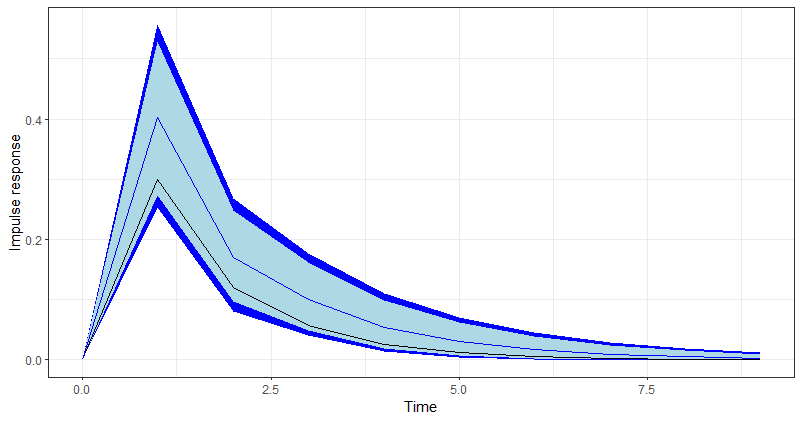
\includegraphics[width=340pt, height=200pt]{Chapters/chapter8/figures/IR23}
	\caption[List of figure caption goes here]{Forecast error impulse response: Response in $y_{2t}$ to shock in $\mu_{3t}$.}\label{fig7}
\end{figure}


\end{enumerate}